\section{Interface utilisateur}%
\label{sec.results.interface}

Dans l'absence d'un système d'\gls{asr}, 
il est impossible de créer un système \foreignlanguage{english}{text-to-speech} complet.
Une autre interface est donc nécessaire pour utiliser le modèle.
Pour cette fin, nous avons développé une interface web de traduction.

\begin{figure}[hbt]
    \begin{center}
        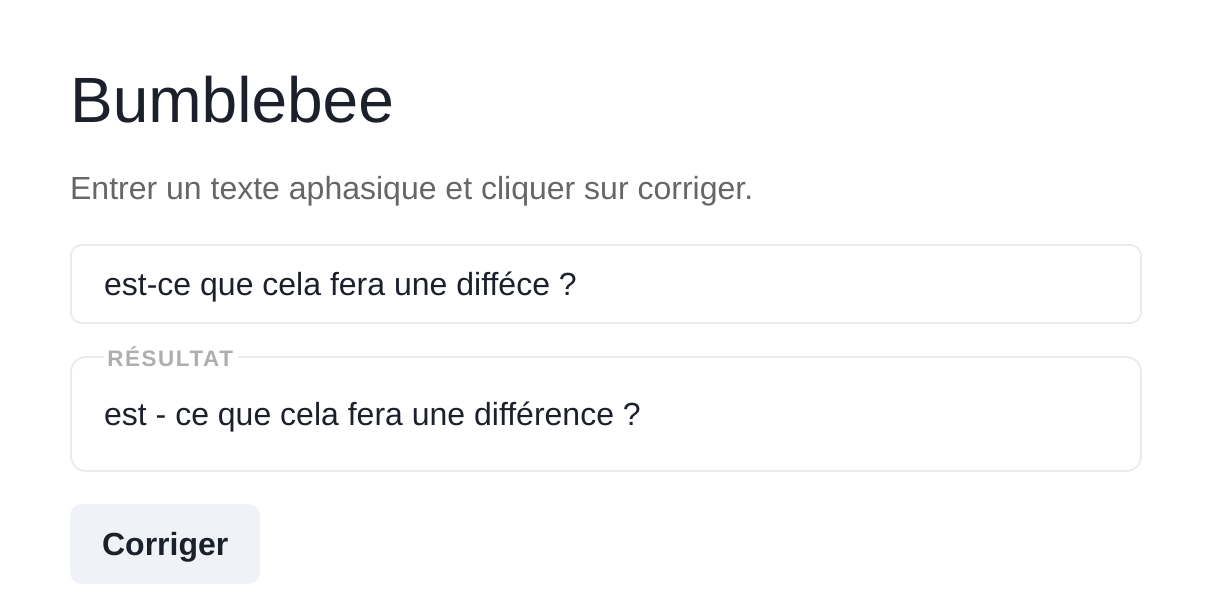
\includegraphics[width=\linewidth]{assets/images/interface.png}
    \end{center}
    \caption{Interface web de traduction.}%
    \label{fig.interface}
\end{figure}

La Figure~\ref{fig.interface} montre l'interface que nous avons développée.
Nous l'avons nommée \textit{Bumblebee}%
\footnote{Une référence à un personnage de la série \textit{Transformers} qui souffre de mutisme, 
mais qui reprend la parole.}.
L'utilisateur peut saisir un texte aphasique dans la zone de texte en haut 
et cliquer sur le bouton \textit{Corriger}.
La correction s'affiche dans la zone de texte en bas.
La figure montre un exemple de correction pour la phrase : ``\textit{est-ce que cela fera une différence ?}''
où le mot ``\textit{différence}'' est remplacé par ``\textit{difféce}''.